\subsection{Wings} %Martina
\noindent Naiad has a pair of wings which are located on the sides of the front. These serve the purpose of hiding the thrusters and to ensure that Naiad moves nicely in the water. According to the thruster specifications, the thrusters need to be re-greased after each use. This means that the wings also need to be removed from the hull after every use, as they cover the screws that needs to be removed for re-greasing. With this in mind, the wings were redesigned with the intent of making them as easy as possible to remove while not harming the hull. Many possible solutions were discussed and almost every idea included splitting the wings into a top and a bottom part, but had different methods of how to secure the wings to the hull. 

One design involved using magnets for attaching the wings to the hull and also using a magnet to attach the two wing parts together. This would make it very easy to remove and reattach the wings. Also, if using the right magnets, they would be able to keep the wings firmly to the hull and not risk them falling off. Furthermore, there would be no need to drill holes in the hull for attaching threads, reducing the risk of breaking the hull in the form of cracks in the plastic or the point force from the weight of the wings on a few small areas of the hull. 

Another solution was to attach the wing parts with screws onto the hull by the use of threads and having a screw or magnet for attaching the two parts together. The bottom part would then be secured to the hull and only the top part would be removed when re-greasing.

 The latter solution was also the final solution, where the two parts would be connected to eachother with magnets to make it easier to remove and attach the top part.

	\subsubsection{Hydrophones}

Naiad will use four hydrophones. Two of them will be placed on each wing, one in the right wing and the other one on the left, and the other two will be placed in the back of the tool plate. 

The hydrophone will be screwed to a box, see fig. \ref{hydrobox} below, and then the box will be screwed to the bottom part of the wing. The idea is to make the hydrophones easy to remove and easy to mount. 

	\begin{figure}[!ht]
	\begin{center}
		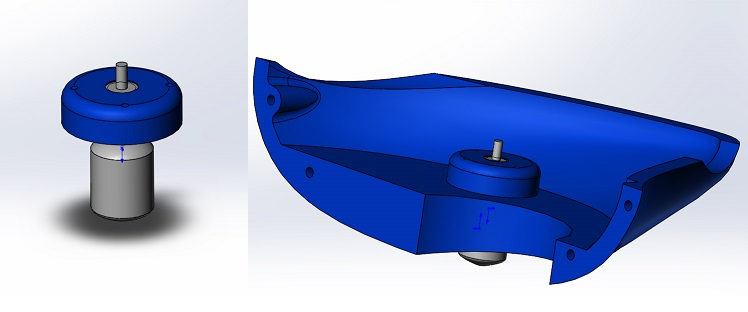
\includegraphics[width=150mm]{./Images/Mechanics/Hydrobox.JPG}
		\caption{The first picture shows the hydrophone attached to the box. The second picture shows the box attached to the bottom part of the wing.}
		\label{hydrobox}
	\end{center}
\end{figure}

	\subsubsection{Coloured status LEDs}
\noindent It was decided that LEDs should be added to the wings of Naiad for the purpose of showing different status of what is going on by using colour codes. The final design consists of a box which fits a PMMA plastic tubes with LEDs in them. This box is integrated into the wings and the top part has the same shape as the wing. 
fig. \ref{hejhej} shows the LED box itself and fig. \ref{hejhejs} shows the box integrated into the wing. 

\begin{figure}[!ht]
	\begin{center}
		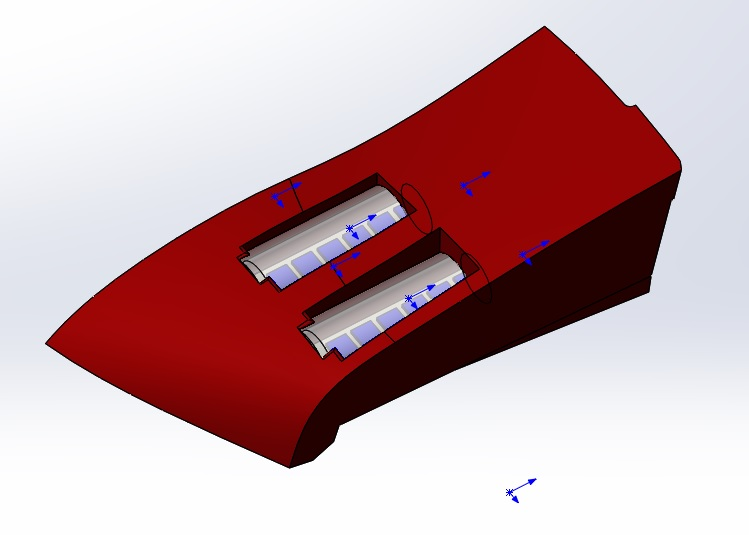
\includegraphics[width=80mm]{./Images/Mechanics/LED_box_with_LEDS.jpg}
		\caption{The LED box separated from the wing.}
		\label{hejhej}
	\end{center}
\end{figure}

\begin{figure}[!ht]
	\begin{center}
		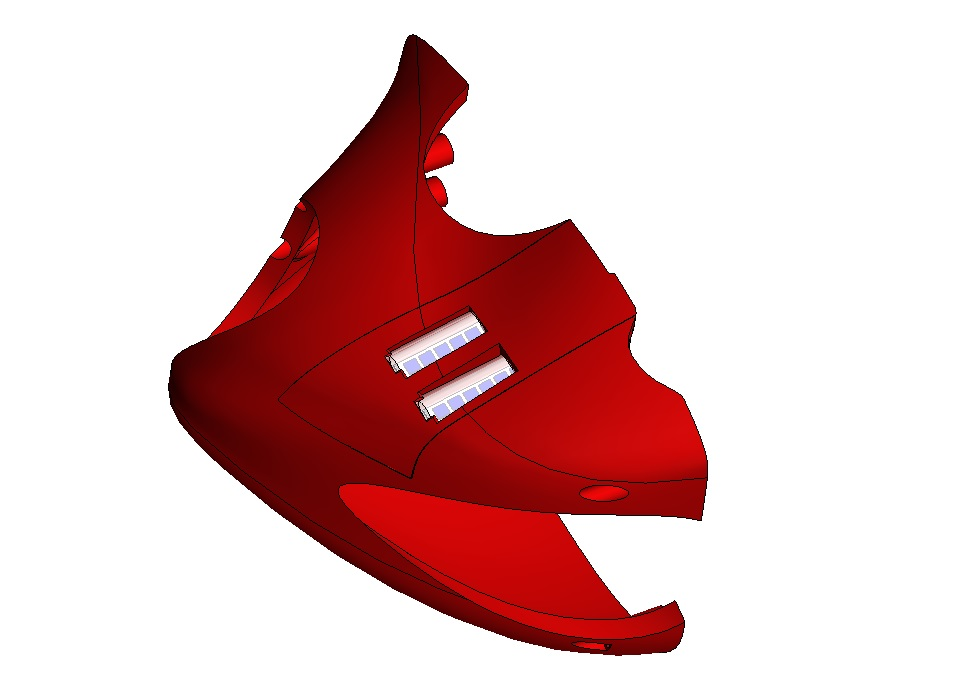
\includegraphics[width=80mm]{./Images/Mechanics/Right_Wing_with_LED_box.jpg}
		\caption{The LED box merged with the wing.}
		\label{hejhejs}
	\end{center}
\end{figure}
